\documentclass{beamer}
 
\usepackage[utf8]{inputenc}

\usetheme{Madrid}
\usecolortheme{default}

\usepackage[qm]{qcircuit}
\usepackage{bibentry}




\usepackage{tikz,tikz-cd}












\usepackage{physics}
\usepackage{amsmath}
\usepackage{amsfonts}
\usepackage{esint}
\usepackage{bbold}
\usepackage{mathtools}
\usepackage{dsfont}
\usepackage{amsthm}
\usepackage{bbm}
\usepackage{amssymb}
\theoremstyle{definition}
\newtheorem{defn}{Definition}[section]
\newtheorem{prop}{Properties}[section]
\newtheorem{rmk}{Remark}[section]
\newtheorem{exmp}{Example}[section]
\newtheorem{prob}{Problem}[section]
\newtheorem{sln}{Solution}[section]
\newtheorem{thm}{Theorem}[section]
\newtheorem*{prob*}{Problem}
\newtheorem*{sln*}{Solution}
\usepackage{empheq}
\usepackage{tensor}
\usepackage{hyperref}
\usepackage{xcolor}

\newcommand{\R}{\mathbb{R}}
\newcommand{\F}{\mathcal{F}}
\newcommand{\p}{\partial}

\newcommand{\V}{\mathbf{V}}
\newcommand{\W}{\mathbf{W}}
\newcommand{\Z}{\mathbf{Z}}
\newcommand{\Y}{\mathbf{Y}}
\newcommand{\U}{\mathbf{U}}
\newcommand{\X}{\mathbf{X}}

\newcommand{\A}{\mathcal{A}}
\newcommand{\B}{\mathcal{B}}

\newcommand{\xpan}{\text{span}}

\newcommand{\lag}{\mathcal{L}}

\newcommand{\J}{\mathbf{J}}

\newcommand{\M}{\mathcal{M}}

\newcommand{\K}{\mathcal{K}}

\newcommand{\N}{\mathcal{N}}

\newcommand{\E}{\mathcal{E}}

\newcommand{\ima}{\text{Im}}
\newcommand{\lin}{\overset{\text{linear}}{\longrightarrow}}
\newcommand{\T}{\mathcal{T}}
\newcommand{\poly}{\mathbb{P}}
\newcommand{\s}{\mathcal{S}}

\newcommand{\gives}{\rotatebox[origin=c]{180}{$\Rsh$}	}


\newcommand{\bigzero}{\mbox{\normalfont\Large\bfseries 0}}
\newcommand{\rvline}{\hspace*{-\arraycolsep}\vline\hspace*{-\arraycolsep}}




 
 
%Information to be included in the title page:
\title{Matrices in Quantum Computing}
\author[Huan Q. Bui] % (optional)
{Huan Q. Bui}

\institute[Colby College] % (optional)
{
	
	Matrix Analysis
	\and
	Professor Leo Livshits
}
\date{CLAS, May 2, 2019}
 
%\logo{
\includegraphics[height=0.3cm]{colby.png}}
 
\begin{document}
 
\frame{\titlepage}
 
\begin{frame}
\frametitle{Presentation layout}
\tableofcontents
\end{frame}



\section{Background}



\begin{frame}
\frametitle{Qubits}
\textit{Qubit:} A quantum system with measurable eigenstates $\ket{0}$ and $\ket{1}$,
\begin{figure}[h!]
	\centering
	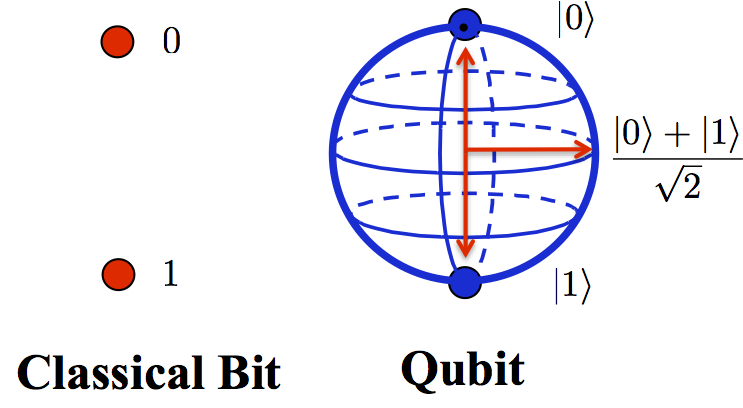
\includegraphics[scale=0.35]{atom1.png}
\end{figure}
\begin{align*}
\ket{0} = \begin{bmatrix}
1\\0
\end{bmatrix}\hspace{0.5cm} \ket{1} = \begin{bmatrix}
0\\1
\end{bmatrix} \hspace{0.5cm} 
%\rightarrow \text{like a Classical Bit.}
\end{align*}
\begin{align*}
&\text{Wavefunction}: \ket{\psi} = a\ket{0} + b\ket{1},\hspace{0.5cm} \abs{a}^2 + \abs{b}^2 = 1.\\
&\,\\
&\text{Probabilistic: } Pr(\ket{\psi} \to \ket{0}) = \abs{a}^2\hspace{0.5cm}
%P(\ket{\psi} \to \ket{1}) = \abs{b}^2.
\end{align*}


\end{frame}




\begin{frame}
\frametitle{Quantum Gates}

\textit{Quantum gate:} linear transformation on $\ket{\psi}$ of one or many qubits. \\
$\,$\\
A common single-qubit quantum gate: Hadamaar gate.
\begin{align*}
 H \stackrel{\Delta}{=}\frac{1}{\sqrt{2}}\begin{bmatrix}
1&1\\1&-1
\end{bmatrix}
\end{align*}
For example, applying $H$ to $\ket{0}$:
\begin{align*}
H\ket{0} = H\begin{bmatrix}
1\\0
\end{bmatrix} = \frac{1}{\sqrt{2}}\begin{bmatrix}
1\\1
\end{bmatrix} = \frac{1}{\sqrt{2}}\ket{0} + \frac{1}{\sqrt{2}}\ket{1}.
\end{align*}

%\begin{align*}
%\text{Control-Not: } CNOT \stackrel{\Delta}{=} \begin{bmatrix}
%1 & 0 & 0 & 0\\
%0 & 0 & 0 & 1\\
%0 & 0 & 1 & 0\\
%0 & 1 & 0 & 0
%\end{bmatrix}.
%\end{align*}

\end{frame}























\section{Motivation}

\begin{frame}
\frametitle{Multiple Qubits}
Like classical circuits, quantum circuits require multiple qubits.\\
$\rightarrow$ How to express the quantum state of two qubits $\ket{\psi_1}\in \V_1, \ket{\psi_2}\in \V_2$?
\begin{align*}
\ket{\psi_1\psi_2} \stackrel{?}{\sim} \ket{\psi_1}, \ket{\psi_2}
\end{align*}
What if there are more than two $\ket{\psi_i}$'s $\in \V_i$'s
\begin{align*}
\ket{\psi_1\psi_2\dots\psi_n} \stackrel{?}{\sim} \ket{\psi_1},\ket{\psi_2},\dots,\ket{\psi_n}?
\end{align*}
Mathematically,
\begin{itemize}
	\item Is there a vector space that contains $\ket{\psi_1\psi_2\dots\psi_n}$?
	\item What is the vector space containing $\ket{\psi_1\psi_2\dots\psi_n}$?
	\item How does $\ket{\psi_1\psi_2\dots\psi_n}$ change w.r.t $\A_1\ket{\psi_1}$ where $\A_1 \in \mathfrak{L}(\V)$?
	\item What about for $\A_1\ket{\psi_1},\dots\A_n\ket{\psi_n}$, where $\A_i \in \mathfrak{L}(\V)$?
\end{itemize}
\end{frame}


















\section{Some Matrix Theory}


\begin{frame}
\frametitle{Tensor Product}
\begin{block}{Postulate (QM): \tiny{\cite{nielsen2002quantum}}}
	The state space of a composite physical system is the \textit{tensor product} of the state spaces of the component physical systems.
\end{block}
For $\ket{\psi_1}\in \V_1, \ket{\psi_2} \in \V_2$, 
\begin{align*}
\ket{\psi_1\psi_2} \in \V_1\otimes   \V_2,
\end{align*}
where the joint state $\ket{\psi_1\psi_2}$ is given by
\begin{align*}
\ket{\psi_1\psi_2} = \ket{\psi_1}\ket{\psi_2} = \ket{\psi_1}\otimes   \ket{\psi_2}.
\end{align*}
%$\ket{\psi_1\dots\psi_n}$ is an \textit{elementary tensor} in $\V_1\otimes \dots \otimes \V_n$. \\
%$\,$\\
%Not all $\ket{\phi} \in \V_1\otimes \dots \otimes \V_n$ are elementary.




\end{frame}





\begin{frame}


\frametitle{Tensor Product: Definition}	

\textbf{What is this ``$\otimes$'' object?}

\begin{block}{Definition \cite{Tor}}
The \textit{tensor product} of $\V$ and $\W$ is a vector space $\V \otimes \W$ with the \textit{bilinear map} $\phi : \V\times \W \longrightarrow \V\otimes \W$, such that for every vector space $\X$ and every bilinear map $f : \V \times \W \longrightarrow \X$, there exists a \textit{unique linear map} $\hat{f} : \V\otimes \W \longrightarrow \X$ such that $f = \hat{f} \circ \phi$.
\end{block}


\begin{block}{In other words...}

Giving the $\hat{f} : \V\otimes \W \lin \X$ is the same as giving $f : \V\times \W \stackrel{\text{bilinear}}{\longrightarrow} \X$.


\end{block}




\end{frame}


\begin{frame}[fragile]
\frametitle{Tensor Product: Construction}
\centering
\begin{center}
\begin{tikzcd}[row sep=15ex, column sep=20ex]
	\V \otimes \W  \arrow[r, "linear"', "\hat{f}"]  & \X
	\\ \V \times \W \arrow[ur, "f", "multilinear"'] \arrow[u, hook, "\phi"]
\end{tikzcd}
\end{center}
\end{frame}








\begin{frame}
\frametitle{Tensor Product: Vectors \tiny{\cite{cern}}}
Let $v_1,\dots,v_n$ be a basis for $\V$ and $w_1,\dots,w_m$ be a basis for $\W$,
\begin{itemize}
	\item $v_i \otimes w_j$'s are elementary.
	\item  
	$\{ v_i \otimes w_j\}$ is a basis of $\V\otimes \W$:
	\begin{align*}
	v\otimes w = \sum^n_i \alpha_i v_i \otimes \sum^m_j \beta_j w_j =  \sum^{n,m}_{i,j}\alpha_i\beta_j(v_i \otimes w_j).
	\end{align*}
	
	\item Not all $x \in \V\otimes \W$ are elementary.
	\item $\dim(\V\otimes \W) = \dim(\V)\dim(\W) = nm$.
\end{itemize}







\end{frame}





\begin{frame}[fragile]
\frametitle{Tensor Product: Operators}
Let $\lag\otimes\M \in \mathfrak{L}(\V\otimes \W)$, where $\lag \in \mathfrak{L}(\V)$, and $\M \in \mathfrak{L}(\W)$. 
%\begin{align*}
%(\lag\otimes\M)(v\otimes w) \stackrel{?}{\sim}\lag(v)\otimes \M(w).
%\end{align*} 

\begin{center}
	\begin{tikzcd}[row sep=9ex, column sep=15ex]
		\V \otimes \W  \arrow[r, "\lag\otimes\M"]  & \V\otimes\W
		\\ \V \times \W \arrow[ur, "\F"'] \arrow[u, hook, "\phi"]
	\end{tikzcd}
\end{center}
$\F(v,w) = \lag(v)\otimes \M(w)$. By uniqueness,
\begin{align*}
%(\lag\otimes \M)\circ \phi = \F \iff
 \boxed{(\lag\otimes \M)(v\otimes w) = \lag(v) \otimes \M(w)}
\end{align*}

\end{frame}

\begin{frame}[fragile]
\frametitle{Tensor Product to Kronecker Product}
Let $\Gamma$ be a basis for $\V\otimes \W$, and $\{\,\}_\Gamma = \A^{-1}_\Gamma$ is the coordinatization from $\V\otimes \W$ to $\mathbb{C}^{nm}$, where $n = \dim(\V), m = \dim(\W)$.
\begin{center}
	\begin{tikzcd}[row sep=15ex, column sep=20ex]
		\V \otimes \W  \arrow[r, "linear"', "\lag\otimes \mathcal{M}"] \arrow[d, "\{\,\}_\Gamma"] & \V\otimes \W
		\\ \mathbb{C}^{nm}   \arrow[r, "linear"', "\{\lag\otimes \mathcal{M}\}_{\Gamma\leftarrow\Gamma}"] & \mathbb{C}^{nm}  \arrow[u, "\A_\Gamma"]
	\end{tikzcd}
\end{center}
\end{frame}


\begin{frame}
\frametitle{Kronecker Product}
\begin{align*}
[\lag\otimes\M]_{\Gamma\leftarrow\Gamma} = [\lag]_{\Gamma\leftarrow\Gamma}\otimes [\M]_{\Gamma\leftarrow\Gamma}.
\end{align*}
If 
\begin{align*}
[\lag]_{\Gamma\leftarrow\Gamma} = \begin{bmatrix}
l_{11} & l_{12}\\l_{21}&l_{22}
\end{bmatrix}\hspace{0.5cm}\text{and}\hspace{0.5cm}
[\M]_{\Gamma\leftarrow\Gamma} = \begin{bmatrix}
m_{11} & m_{12}\\m_{21}& m_{22}
\end{bmatrix}
\end{align*}
then the \textit{Kronecker product} $[\lag]_{\Gamma\leftarrow\Gamma} \otimes [\M]_{\Gamma\leftarrow\Gamma} $ is defined as
\begin{align*}
[\lag]_{\Gamma\leftarrow\Gamma}\otimes [\M]_{\Gamma\leftarrow\Gamma} &= \begin{bmatrix}
l_{11}\M& l_{12}\M \\ l_{21}\M& l_{22}\M 
\end{bmatrix}\\
&= \begin{bmatrix}
l_{11}\begin{bmatrix}
m_{11} & m_{12}\\m_{21}& m_{22}
\end{bmatrix}& l_{12}\begin{bmatrix}
m_{11} & m_{12}\\m_{21}& m_{22}
\end{bmatrix} \\ l_{21}\begin{bmatrix}
m_{11} & m_{12}\\m_{21}& m_{22}
\end{bmatrix}& l_{22}\begin{bmatrix}
m_{11} & m_{12}\\m_{21}& m_{22}
\end{bmatrix}
\end{bmatrix}.
\end{align*}
\end{frame}



%
%\begin{frame}
%\frametitle{Why Tensor Product?}
%
%\end{frame}







\begin{frame}
\frametitle{Kronecker Product}
Doesn't care where scalar goes...
$$ (\alpha \A) \otimes \B = \A \otimes (\alpha \B) = \alpha(\A \otimes \B)$$
Associative: $$(\A \otimes \B) \otimes \mathcal{C} = \A \otimes (\B \otimes \mathcal{C})$$
Left-distributive: $$\A \otimes (\B + \mathcal{C}) = \A\otimes \B + \A \otimes \mathcal{C}$$
Right-distributive: $$(\A + \B)\otimes \mathcal{C} = \A \otimes \mathcal{C} + \B \otimes \mathcal{C}$$

Not commutative.
\end{frame}





%\begin{frame}
%\frametitle{Tensor Products: more basic properties}
%Other properties:
%\begin{itemize}
%	\item Bilinear: linear in both arguments.
%	\item Associative
%	\item Distributive
%	
%	\item $(\A \otimes \B)^\dagger = \A^\dagger \otimes \B^\dagger$.
%	\item $\Tr(\A\otimes \B) = \Tr(\A)\cdot \Tr(\B)$.
%	\item $\det(\A \otimes \B) = (\det(\A))^m\cdot \det(\B)^n$, where $m = \text{size}(\A), n =\text{size}(\B)$. 
%\end{itemize}
%\end{frame}




















\section{Example: A 2-Qubit Entangler}






\begin{frame}
\frametitle{Multiple Qubits with Kronecker Product}
\underline{Example}: Representing 2-qubits with the Kronecker Product:
\begin{align*}
&\ket{01} = \ket{0} \otimes \ket{1} = \begin{bmatrix}
1\\0
\end{bmatrix}\otimes 
\begin{bmatrix}
0\\1
\end{bmatrix}
=
\begin{bmatrix}
1\begin{bmatrix}
0\\1
\end{bmatrix}\\
0\begin{bmatrix}
0\\1
\end{bmatrix}
\end{bmatrix} = \begin{bmatrix}
0\\1\\0\\0
\end{bmatrix}\\
&\ket{00} = \ket{0} \otimes \ket{0} = \begin{bmatrix}
1\\0
\end{bmatrix}\otimes 
\begin{bmatrix}
1\\0
\end{bmatrix}
=
\begin{bmatrix}
1\begin{bmatrix}
1\\0
\end{bmatrix}\\
0\begin{bmatrix}
1\\0
\end{bmatrix}
\end{bmatrix} = \begin{bmatrix}
1\\0\\0\\0
\end{bmatrix}\\
&\ket{10} = \begin{bmatrix}
0&0&1&0
\end{bmatrix}^\top\\ &\ket{11} = \begin{bmatrix}
0&0&0&1
\end{bmatrix}^\top.
\end{align*}
$\rightarrow \ket{00}, \ket{01}, \ket{10}, \ket{11}$ form a basis for a 2-qubit system.
\end{frame}

\begin{frame}
\frametitle{Entangling 2 qubits}
\begin{itemize}
	\item Entanglement. 
	\item Recipe.
	\item Running on IBM-Q.
\end{itemize}
\end{frame}


\begin{frame}
\frametitle{Entanglement}
Not every $\ket{\psi} \in \V\otimes \W$ is an elementary tensor.  \\
$\,$\\
\underline{Example}: There are no states $\ket{c}, \ket{d} \in \mathbb{C}^2$ such that
\begin{align*}
\ket{c} \otimes \ket{d}  &= \begin{bmatrix}
\frac{1}{\sqrt{2}} & 0 & 0 & \frac{1}{\sqrt{2}}
\end{bmatrix}^\top \\
&= \frac{1}{\sqrt{2}}\ket{00} + \frac{1}{\sqrt{2}}\ket{11} \textbf{$\rightarrow$ Entangled}
\end{align*}
\underline{Examples}: Bell states, also entangled \cite{Bell}
\begin{align*}
\frac{1}{\sqrt{2}}\ket{00} - \frac{1}{\sqrt{2}}\ket{11}\\
\frac{1}{\sqrt{2}}\ket{01} + \frac{1}{\sqrt{2}}\ket{10}\\
\frac{1}{\sqrt{2}}\ket{01} - \frac{1}{\sqrt{2}}\ket{10}\\
\end{align*}


\end{frame}

\begin{frame}
\frametitle{``Entangled'' operators}
\textit{For operators:} $\A \in \mathfrak{\lag}(\V), \mathcal{B} \in \mathfrak{\lag}(\W)$, $\A\otimes \B \in \mathfrak{\lag}(\V \otimes \W)$ is defined by
\begin{align*}
(\A \otimes \B)(\ket{v}\otimes \ket{w}) = (\A\ket{v})\otimes (\B\ket{w}).
\end{align*}
Not all $C \in \mathfrak{\lag}(\V\otimes \W)$ can be written as $\A \otimes \B$, $\A \in \mathfrak{\lag}(\V), \mathcal{B} \in \mathfrak{\lag}(\W)$.\\
$\,$\\
\underline{Example}:
\begin{align*}
CNOT_2 = \begin{bmatrix}
1&0&0&0\\
0&0&0&1\\
0&0&1&0\\
0&1&0&0
\end{bmatrix} \hspace{0.5cm}
\begin{cases}
\ket{00} \to \ket{00}\\
\ket{10} \to \ket{10}\\
\ket{01} \to \ket{11}\\
\ket{11} \to \ket{01}
\end{cases}
%\hspace{0.5cm}
%SWAP = 
%\begin{bmatrix}
%1&0&0&0\\
%0&0&1&0\\
%0&1&0&0\\
%0&0&0&1
%\end{bmatrix} 
\end{align*}
\end{frame}




\begin{frame}
\frametitle{2-Qubit Entanglement Circuit}{\cite{eastin2004q}}
\begin{center}
	$\,$\Qcircuit @C=.7em @R=.4em  {
		\lstick{a: \ket{0}} & \qw & \qw & \targ & \meter & \qw \\
		\lstick{b: \ket{0}} & \qw & \gate{H} & \ctrl{-1}& \meter & \qw 
	}
\end{center}
\begin{align*}
H\begin{bmatrix}
1\\0
\end{bmatrix}_b = \frac{1}{\sqrt{2}}\begin{bmatrix}
1&1\\1&-1
\end{bmatrix}\begin{bmatrix}
1\\0
\end{bmatrix}_b = \frac{1}{\sqrt{2}}\ket{0}_b + \frac{1}{\sqrt{2}}\ket{1}_b
\end{align*}
\begin{align*}
CNOT_b = C_b = \begin{bmatrix}
1&0&0&0\\
0&0&0&1\\
0&0&1&0\\
0&1&0&0
\end{bmatrix}\hspace{0.5cm}
\begin{cases}
\ket{00} \to \ket{00}\\
\ket{10} \to \ket{10}\\
\ket{01} \to \ket{11}\\
\ket{11} \to \ket{01}
\end{cases}
\end{align*}
\end{frame}


\begin{frame}
\frametitle{Entanglement (cont.)}
\begin{center}
	$\,$\Qcircuit @C=.7em @R=.4em  {
		\lstick{a: \ket{0}} & \qw & \qw & \targ & \meter & \qw \\
		\lstick{b: \ket{0}} & \qw & \gate{H} & \ctrl{-1}& \meter & \qw 
	}
\end{center}
One way to see how this works...
\begin{align*}
CNOT_b\left(I  \begin{bmatrix}
1\\0
\end{bmatrix}_a
\otimes
H\begin{bmatrix}
1\\0
\end{bmatrix}_b
\right)
&= CNOT_b\left(\begin{bmatrix}
1&0\\0&1
\end{bmatrix}\begin{bmatrix}
1\\0
\end{bmatrix}_a\otimes \frac{1}{\sqrt{2}}\begin{bmatrix}
1&1\\1&-1
\end{bmatrix}\begin{bmatrix}
1\\0
\end{bmatrix}_b\right)\\
&=
CNOT_b
\begin{bmatrix}
1/\sqrt{2}\\1/\sqrt{2}\\0\\0
\end{bmatrix}
= 
\begin{bmatrix}
1/\sqrt{2}\\0\\0\\1/\sqrt{2}
\end{bmatrix}\\ &= \frac{1}{\sqrt{2}}\ket{0}\otimes\ket{0} + \frac{1}{\sqrt{2}}\ket{1}\otimes\ket{1}\\
&\rightarrow \textbf{Entangled}
\end{align*}
\end{frame}







\begin{frame}
\frametitle{Entanglement (cont.)}
Another way to see how this works...
\begin{align*}
CNOT_b\left[(I\ket{0}) \otimes (H_b\ket{0})\right] &= CNOT_b(I \otimes H_b)(\ket{0} \otimes \ket{0}) \\
%\begin{bmatrix}
%1\\0
%\end{bmatrix}
%\otimes
%\frac{1}{\sqrt{2}}
%\begin{bmatrix}
%1&1\\1&-1
%\end{bmatrix}
%\begin{bmatrix}
%1\\0
%\end{bmatrix}
&=
CNOT_b\begin{bmatrix}
\frac{1}{\sqrt{2}}\begin{bmatrix}
1&1\\
1&-1
\end{bmatrix}& \mathcal{O}\\
\mathcal{O} & \frac{1}{\sqrt{2}}\begin{bmatrix}
1&1\\1&-1
\end{bmatrix}
\end{bmatrix}\begin{bmatrix}
1\\0\\0\\0
\end{bmatrix}\\
%\begin{bmatrix}
%\frac{1}{\sqrt{2}} & \frac{1}{\sqrt{2}} & 0&0
%\end{bmatrix}^\top 
&= CNOT_b\begin{bmatrix}\frac{1}{\sqrt{2}} & \frac{1}{\sqrt{2}} & 0&0
\end{bmatrix}^\top \\
&= \begin{bmatrix}\frac{1}{\sqrt{2}} & 0 & 0& \frac{1}{\sqrt{2}}
\end{bmatrix}^\top
\end{align*}
%$\rightarrow$ Possible to write $H$ as $I \otimes H_b$. Not possible for $CNOT_b$.
\end{frame}







\section{Simulation on IBM-Q}


\begin{frame}
\frametitle{Simulation on IBM-Q}

Entanglement circuit, revisited

\begin{center}
	$\,$\Qcircuit @C=.7em @R=.4em  {
		\lstick{a: \ket{0}} & \qw & \qw & \targ & \meter & \qw \\
		\lstick{b: \ket{0}} & \qw & \gate{H} & \ctrl{-1}& \meter & \qw 
	}
	
	\begin{figure}[h!]
		\centering
		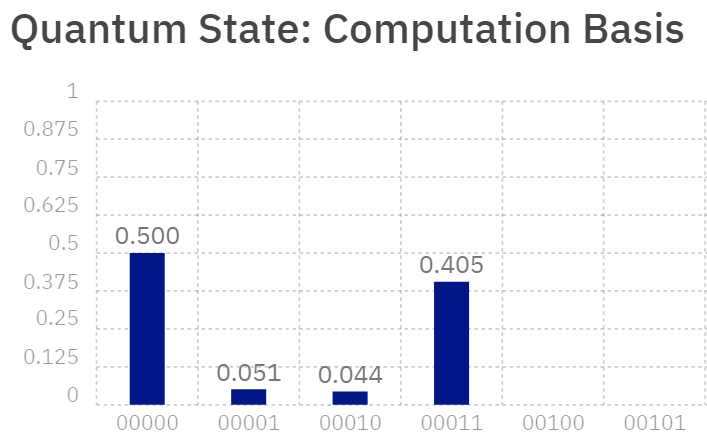
\includegraphics[scale=0.7]{ibmq}
	\end{figure}
\end{center}


\end{frame}















\section{Recap}

\begin{frame}
\frametitle{Recap}

\begin{itemize}
\item Representing multi-qubit systems with tensor products.
\item Representing multi-qubit operators with tensor products.
\item Compute with the Kronecker product.
\item Entanglement, mathematically.
\item 2-qubit entangler, mathematically.
\item Entanglement on IBM-Q.
\end{itemize}

\end{frame}

\begin{frame}
\frametitle{References}



\bibliographystyle{amsalpha}
\bibliography{references}{}



\end{frame}





























































%\begin{frame}
%\frametitle{Qubits \& Quantum Gates}
%\textit{Qubit:} A quantum system with two measurable physical states $\ket{0}$ and $\ket{1}$,
%\begin{align*}
%\ket{0} = \begin{bmatrix}
%1\\0
%\end{bmatrix}\hspace{0.5cm} \ket{1} = \begin{bmatrix}
%0\\1
%\end{bmatrix}.
%\end{align*}
%Before measurement,
%\begin{align*}
%\ket{\psi} = a\ket{0} + b\ket{1} \in \mathbb{C}^2,\hspace{0.5cm} \abs{a}^2 + \abs{b}^2 = 1.
%\end{align*}
%
%Physically,
%\begin{align*}
%P(\ket{\psi} \to \ket{0}) = \abs{a}^2\hspace{0.5cm}
%P(\ket{\psi} \to \ket{1}) = \abs{b}^2.
%\end{align*}
%
%\textit{Quantum gate:} a unitary transformation on $\ket{\psi}$. 
%\end{frame}

%\begin{frame}
%\frametitle{Qubits \& Quantum Gates}
%
%\textit{Multiple Qubits}: A $k$-qubit state is linear combination of
%\begin{align*}
%\ket{x_1\dots x_k} = \ket{x_1}\otimes \dots \otimes \ket{x_k} \in \otimes^k \mathbb{C}^2, \hspace{0.5cm} x_i \in \{0,1\}.
%\end{align*}
%``$\otimes$'' on vectors/matrices: \textbf{Kronecker product}. If $\A \in \mathbb{M}_{m\times n}$ and $\B \in \mathbb{M}_{p\times q}$, then
%\begin{align*}
%\A \otimes \B = \begin{bmatrix}
%a_{11}\B & \dots & a_{1n}\B\\
%\vdots & \ddots & \vdots\\
%a_{m1}\B & \dots & a_{mn}\B
%\end{bmatrix} \in \mathbb{M}_{mn \times pq}.
%\end{align*}
%\end{frame}
















%\begin{frame}
%\frametitle{Tensor Products}
%The \textit{tensor product} of $\V = \mathbb{C}^{\Sigma_1}$ and $\W = \mathbb{C}^{\Sigma_2}$ is
%\begin{align*}
%\V \otimes \W = \mathbb{C}^{\Sigma_1 \times \Sigma_2}.
%\end{align*}
%\textit{Elementary tensors} span $\V\otimes \W$. For $\ket{v} \in \V$ and $\ket{w} \in \W$, 
%\begin{align*}
%\ket{v}\otimes \ket{w}\equiv \ket{v}\ket{w} \equiv \ket{vw}  \in \V \otimes \W.
%\end{align*} 
%
%\underline{Example}: Representing the classical number ``1'' with two qubits:
%\begin{align*}
%1_2 \equiv \ket{01} = \ket{0} \otimes \ket{1} = \begin{bmatrix}
%1\\0
%\end{bmatrix}\otimes 
%\begin{bmatrix}
%0\\1
%\end{bmatrix}
%=
%\begin{bmatrix}
%1\begin{bmatrix}
%0\\1
%\end{bmatrix}\\
%0\begin{bmatrix}
%0\\1
%\end{bmatrix}
%\end{bmatrix} = \begin{bmatrix}
%0\\1\\0\\0
%\end{bmatrix}.
%\end{align*}
%
%
%\end{frame}











%\begin{frame}
%\frametitle{Tensor Products (cont.)}
%
%$\xpan(\ket{00}, \ket{01}, \ket{10}, \ket{11}) = \V\otimes \W$, where
%\begin{align*}
%\ket{00} = \begin{bmatrix}
%1&0&0&0
%\end{bmatrix}^\top, \ket{10} = \begin{bmatrix}
%0&0&1&0
%\end{bmatrix}^\top, \ket{11} = \begin{bmatrix}
%0&0&0&1
%\end{bmatrix}^\top.
%\end{align*}
%Linear independence $\rightarrow$ $(\ket{00}, \ket{01}, \ket{10}, \ket{11})$ form a computational basis. \\
%$\,$\\
%A \textit{generic state}: For $\abs{a_{00}}^2 + \abs{a_{01}}^2 + \abs{a_{10}}^2 + \abs{a_{11}}^2 = 1$,
%\begin{align*}
%\ket{\psi} = a_{00}\ket{00} + a_{01}\ket{01} + a_{10}\ket{10} + a_{11}\ket{11}.
%\end{align*}
%
%\end{frame}







%\begin{frame}
%\frametitle{$SWAP \neq S_1 \otimes S_2$}
%Consider the 2-qubit $SWAP$ map:
%\begin{align*}
%SWAP = 
%\begin{bmatrix}
%1&0&0&0\\
%0&0&1&0\\
%0&1&0&0\\
%0&0&0&1
%\end{bmatrix} \in \lag(\V\otimes \W).
%\end{align*}
%Observe: 
%\begin{align*}
%SWAP(\ket{0}\otimes \ket{1}) = \ket{1}\otimes \ket{0}.
%\end{align*}
%Suppose for $S_1 \in \lag(\V), S_2 \in \lag(\W)$
%\begin{align*}
%SWAP = S_1 \otimes S_2
%\end{align*}
%\end{frame}





























 
\end{document}
